\section{Motivation and Background}
\label{sec:background}

Over the last decade single GPU performance has scaled well due to a 
significant growth in per-GPU transistor count and DRAM bandwidth. For example, 
in 2010 Nvidia's Fermi GPUs integrated 1.95B transistors on a 
529mm\textsuperscript{2} die, with 180GB/s of DRAM bandwidth.  In 2016 Nvidia's 
Pascal GPUs contained 12B transistors on a 610 mm\textsuperscript{2} die, while 
relying on 720GB/s of main memory bandwidth. Unfortunately transistor density is 
slowing significantly and vendors are not providing roadmaps beyond 7nm. 
Moreover, GPU die sizes which have been also increasing generationally, are 
expected to slow down due to limitations in lithography and manufacturing cost.

\begin{figure}[t] 
    \centering
    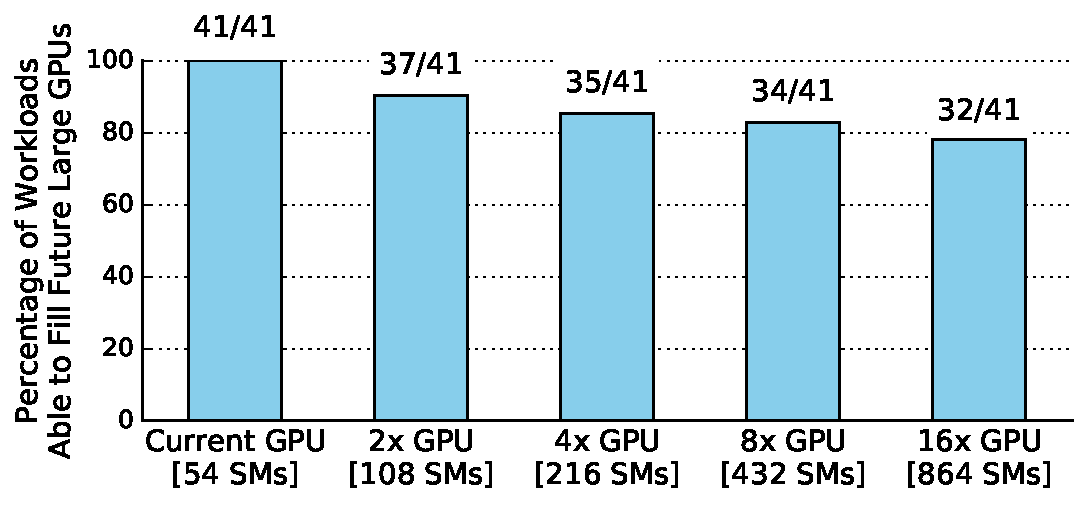
\includegraphics[width=1.0\columnwidth]{figures/plot_ctas_per_sm.pdf}
    \caption{Percentage of benchmarks that have more CTAs on average than 
available SMs.}
    \label{fig:ctas}
\end{figure}

Without either larger or denser dies, manufacturers must turn towards 
alternative solutions to significantly increase GPU performance.  Recently 3D 
die-stacking has seen significant interest due to its successes in the high 
bandwidth DRAM design space~\cite{HBM}. Unfortunately 3D die-stacking still has 
a significant number of engineering challenges related to power delivery, 
energy density, and cooling~\cite{verbree2010cost} when employed in power 
hungry, maximal die-sized chips such as GPUs. Thus we believe GPU manufacturers 
are likely to re-examine a tried and trued solution from CPU world, 
\textit{multi-socket GPUs}, to scaling GPU performance while maintaining the 
current ratio of floating point operations per second (FLOPS) and DRAM 
bandwidth.

Multi-socket GPUs are enabled by the evolution of GPUs from PCIe attached 
peripheral to the primary computing component at system design time.  As a 
result, these GPU optimized systems employ custom PCB designs that accommodate 
high pin count socketed GPUs~\cite{dgx} with inter-GPU interconnects resembling 
QPI or Hypertransport~\cite{NVLINK,INTELQPI,AMDHT}.  However, despite the rapid 
improvement in hardware capabilities, these GPU optimized systems have 
thus far exposed the GPUs in the system as individually addressable GPUs. These
multi-GPU systems can provide high aggregate throughput, for multiple concurrent
GPU accelerated programs, but to accelerate a single GPU program they
require layering additional software runtimes on top of native GPU programming 
interfaces such as CUDA or openCL~\cite{CUDA,OPENCL}. By requiring significant
application re-design many applications are never ported to take advantage
of multiple GPUs.

While extending single GPU application performance significantly is a laudable
goal, we must first understand if applications will be able to leverage future
larger GPUs.  Today NVIDIA's largest GPUs contain 54 SMs with growth to 64 SMs
likely as the product line matures. Across a benchmark set of 41 applications,
later described in Section~\ref{sec:methodology} and Table~\ref{tab:numctas},
we find that many single-GPU optimized workloads contain enough data 
parallelism 
to fill future GPUs that may be 2, 4, or 8$\times$ larger than today's biggest
GPUs.  While single-GPU optimized applications are unlikely to scale to tens
of thousands of GPUs across an entire data center, for the majority of GPU
programs written today we believe there will be significant demand for GPUs that
can scale application performance by as much as a factor of 8$\times$ 
while requiring no additional software engineering.

To understand the performance scalability of a multi-socket NUMA GPU we examine 
the performance that a future 4-socket GPU can achieve while executing 
workloads optimized for a modern single GPU. Not surprisingly, when executing 
uniform memory access (UMA) optimized GPU programs on a highly NUMA GPU, 
performance does not scale well.  We identify that despite software 
optimizations for locality, interconnect bandwidth in a NUMA GPU is still the 
primary limiter on scalable performance.  To overcome this bottleneck we propose 
two classes of improvements that leverage application phasing to reduce the 
observed NUMA penalty.  First, in Section~\ref{sec:interconnect} we examine the 
ability of switch connected GPUs to dynamically change their ingress and egress 
links from symmetric bandwidth provisioning to asymmetric bandwidth 
provisioning.  By using existing interconnects more efficiently the effective 
NUMA bandwidth ratio of remote memory to local memory decreases, improving 
performance.

Second, we propose that to minimize traffic on oversubscribed communication 
links GPU caches need to become NUMA-aware.  Traditional on-chip caches are 
optimized to maximize overall hitrate, thus minimizing off-chip bandwidth.  When 
on-chip caches are backed by a single memory system, or even two symmetric 
memory systems, maximizing hitrate is the best objective function for cache 
policy.  However, in highly NUMA systems,  not all cache misses have the same 
relative cost.  Specifically, due to the NUMA penalty of accessing remote 
memory, overall application throughput may be maximized by preferencing cache 
capacity (and thus improving hit rate) towards data that resides in remote NUMA 
zones rather than faster local memory. To this end, we propose new NUMA-aware 
GPU caches that dynamically skew cache capacity when it is detected that either 
the remote or local memory bandwidth is oversubscribed.

By architecting NUMA-aware GPUs we show that single-GPU application performance 
can be scaled up significantly before costly application re-writes may be 
required. For existing systems like Nvidia's 8-GPU DGX 
Supercomputer~\cite{dgx}, applications which execute on, at most, one GPU could 
see up to an 8$\times$ performance increase transparently, requiring no 
application programmer effort. Before diving into microarchitectural details and 
results, we first describe the transparent multi-socket GPU runtime that enables 
such an architecture.

\begin{figure*}[tp] 
    \centering
    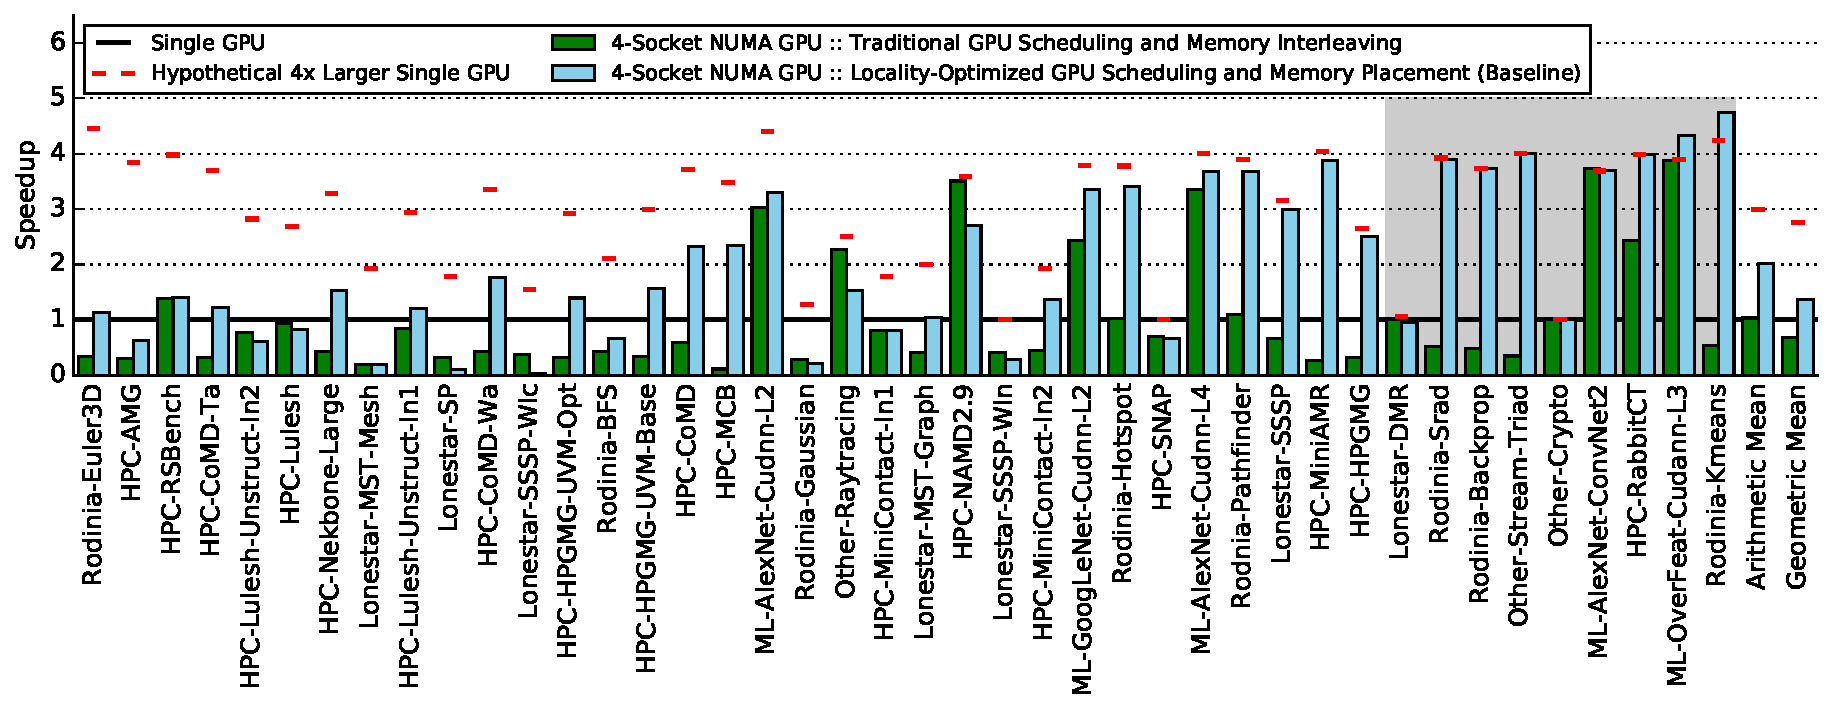
\includegraphics[width=1.0\linewidth]{figures/plot_different_baselines.pdf}
    \caption{Relative performance of a 4-socket NUMA GPU using to a single GPU 
and a hypothetical 4$\times$ larger (all resources scaled) single GPU showing 
upper bound of performance this application can achieve via GPU hardware 
scaling. For the Locality-Optimized design, applications shown in grey 
achieve already 99\% of theoretical scaling (\emph{red dash}) without 
micro-architectural modification.}
    \label{fig:motivation}
\end{figure*}
